\documentclass[titlepage]{article} 
\usepackage{graphicx,lscape,authblk,natbib,fullpage,lineno}
\begin{document}

\linenumbers

\begin{titlepage}
\centering
  
~\vfill

\begin{huge}
  Determining erosion rates in Allchar (Macedonia)\\ to revive the
  lorandite neutrino experiment
\end{huge}

\vfill

\begin{large}
  
\textit{Pieter Vermeesch$^1$, Martin Rittner$^1$,}\\
\textit{Irene Schimmelpfennig$^2$, Lucilla Benedetti$^2$, ASTER Team$^{2,3}$} \\
\vspace{1cm}
$^1$ London Geochronology Centre, Department of Earth Sciences, University College London,\\
Gower Street, London WC1E 6BT, United Kingdom\\
\vspace{0.5cm}
$^2$Aix-Marseille Universit\'{e}, CNRS, IRD, Coll. France, UM 34 CEREGE, \\
Technop\^{o}le de l'Environnement Arbois-M\'{e}diterran\'{e}e, BP 80, \\
13545 Aix-en-Provence, France.\\
\vspace{0.5cm}
$^3$consortium: Georges Auma\^{i}tre, Didier Bourl\`{e}s and Karim Keddadouche\\
\vspace{1cm}
Keywords: cosmogenic nuclides, neutrinos, Macedonia

\end{large}

\vfill
  
\end{titlepage}

%\linenumbers

\begin{abstract}
  \textsuperscript{205}Tl in the lorandite (TiAsS\textsubscript{2})
  mine of Allchar (Majdan, FYR Macedonia) is transformed to
  \textsuperscript{205}Pb by cosmic ray reactions with muons and
  neutrinos.  At depths of $>$300m, muogenic production would be
  sufficiently low for the 4.3~Ma old lorandite deposit to be used as
  a natural neutrino detector.  Unfortunately, the Allchar deposit
  currently sits at a depth of only 120m below the surface, apparently
  making the lorandite experiment technically infeasible.  We here
  present 25 erosion rates estimates for the Allchar area using
  in-situ produced cosmogenic \textsuperscript{36}Cl in carbonates and
  \textsuperscript{10}Be in alluvial quartz. The new measurements
  suggest long term erosion rates of 100-120~m/Ma in the silicate
  lithologies that are found at the higher elevations of the Majdanksa
  River valley, and 200-280~m/Ma in the underlying marbles and
  dolomites. These values indicate that the lorandite deposit has
  spent most of its existence at depths of $>$400m, sufficient for the
  neutrinogenic \textsuperscript{205}Pb component to dominate the muon
  contribution.  Our results suggest that this unique particle physics
  experiment is theoretically feasible and merits further development.
\end{abstract}

\section{Introduction}

When four hydrogen nuclei (protons) fuse to form one helium nucleus in
the solar core, two of them convert to neutrons, releasing two
neutrinos in the process. One of the definitive tests of this
so-called Standard Solar Model is to measure the flux of those
neutrinos. In order to detect these elusive particles, physicists have
devised a number of experiments that broadly fall into two
categories.\\

One group of experiments (Sudbury Neutrino Experiment,
Super-Kamiokande, IceCube, Borexino) measures the light that is
emitted when neutrinos scatter off electrons in water or a
scintillation fluid. A second group (Homestake, Gallex, Sage) measures
the radiation produced by neutrino reaction products such as Ar, Ge,
and B \citep{bahcall1996}. Because neutrino interactions are so rare,
most of these experiments are massive in size and cost, with only one
notable exception.\\

In 1976, Melvin Freedman proposed that the reaction
\textsuperscript{205}Tl ($\nu$,e\textsuperscript{-})
\textsuperscript{205}Pb could form the basis of a natural neutrino
detector with the following advantages over alternative experimental
designs \citep{freedman1976}:

\begin{enumerate}
\item Thanks to the relatively large nuclear cross section of the
  reaction and the 16 Myr half life of \textsuperscript{205}Pb,
  sufficient amounts of the reaction product can accumulate over
  geologic time to be measured by (Shottky) mass spectrometry on a
  sample of just a few kilograms of thallium-bearing minerals such as
  lorandite (TlAsS$_{2}$).
\item The resulting neutrino flux is a long term average over geologic
  time that may be more informative than the snapshot view of solar
  activity provided by artificial detectors.
\item Tl is sensitive to a wider range of neutrino energies than any
  other detector.
\end{enumerate}
    
The world's largest accumulation of Tl-bearing minerals, and the only
one suitable as a neutrino detector, is found in the Allchar mine in
the former Yugoslavian republic of Macedonia. This deposit contains an
estimated 500 tonnes of thallium, mostly in the form of lorandite with
a geologic age of 4.3~Ma \citep{neubauer2009}. In 1983, the
international LOREX (LORandite EXperiment) collaboration was set up
with the aim to investigate the feasibility of Freedman's idea
\citep{pavicevic1988}. It was quickly realised that the Achilles heel
of the proposal was the relatively shallow depth (120m) of the Allchar
mine \citep{neumaier1991}.\\

Besides neutrino reactions, a second production mechanism for
\textsuperscript{205}Pb is by cosmic ray muons. Whereas
\textsuperscript{205}Pb production by neutrinos is effectively
independent of depth, the muon flux decreases exponentially with
depth. But at 120m, the (fast) muon pathway still produces a
significant background signal of \textsuperscript{205}Pb. This paper
shows that the burial depth of the lorandite may have been
significantly greater in the past, because 4.3 million years worth of
erosion may have removed a significant amount of overburden. The
erosion rate, and hence the magnitude of the muogenic
\textsuperscript{205}Pb contribution, may be estimated by analysing
other cosmogenic nuclides such as \textsuperscript{36}Cl and
\textsuperscript{10}Be.\\

In 1991, the steady-state erosion rate of the Allchar area was
estimated by a single \textsuperscript{36}Cl measurement in limestone
\citep{dockhorn1991}. The \textsuperscript{36}Cl concentration was
found to be high, leading to the conclusion that erosion had been
negligible, and that the lorandite had spent most of its 4.3~Ma
lifetime at or near a depth of 120m. This conclusion all but
terminated the geological neutrino detector and the physics community
moved on to other experiments. This paper raises several issues with
the \citet{dockhorn1991} study, suggesting that the lorandite project
may have been aborted prematurely
(Section~\ref{sec:previousstudies}).

\begin{figure}[!ht]
  \centering
  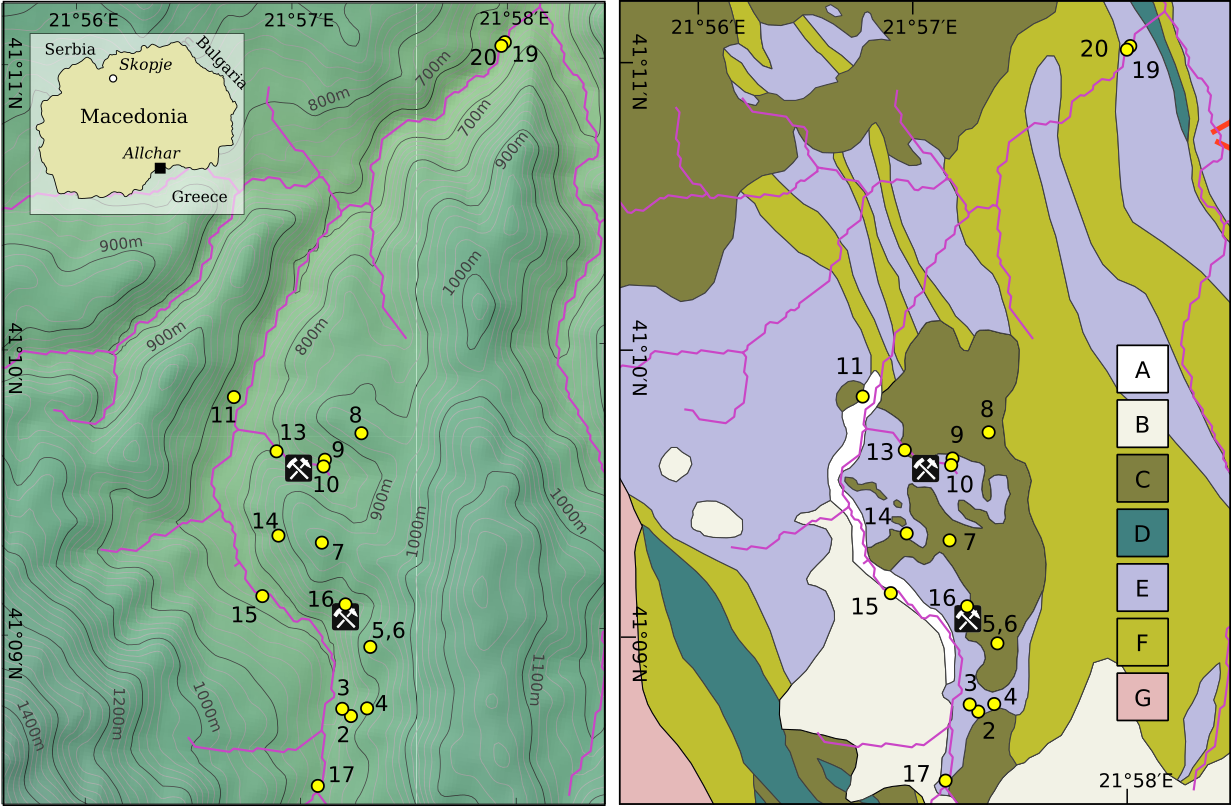
\includegraphics[width=\textwidth]{maps.png}
  \caption{Topographic \citep[left,][]{jarvis2008} and geologic map
    (right) of the Allchar area with indication of the Crven Dol
    (North) and Centralni Deo (South) mine locations, and the sample
    locations (yellow circles). A -- modern alluvium, B -- Quaternary
    sediments, including (fluvio-)glacial deposits, C -- Pliocene
    andesites, rhyolites and tuffs, D -- Jurassic serpentinites, E --
    Triassic limestones and dolomites, F -- Mesozoic sandstones and
    slates, G -- Precambrian gneiss.}
  \label{fig:maps}
\end{figure}

\citet{pavicevic2016} recently conducted a cosmogenic
\textsuperscript{36}Cl -- \textsuperscript{21}Ne --
\textsuperscript{26}Al study to re-evaluate the erosion rates in the
Allchar area. They estimated erosion rates to fall in the 50-100~m/Ma
range, which is much higher than the values obtained by
\citet{dockhorn1991}. Unfortunately, the \citet{pavicevic2016} study
suffers from two methodological issues.  First, it primarily focuses
on the two lorandite-bearing mines (Crven Dol and Centralni Deo,
Figure~\ref{fig:maps}), which were considered to be the most relevant
to the neutrino experiment. These sites also suffer from significant
anthropogenic disturbance. This intrinsically leads to over-estimated
erosion rates. Second, \citet{pavicevic2016} chose not to report any
of their \textsuperscript{10}Be results because ``\textit{the nominal
  erosion rates calculated on the basis of these
  \textsuperscript{10}Be AMS measurements were considerably smaller
  than those obtained on the basis of \textsuperscript{21}Ne,
  \textsuperscript{26}Al, and \textsuperscript{36}Cl
  concentrations}''. We find this line of reasoning to be
questionable, because \textsuperscript{10}Be is generally considered
to be the most reliable and least problematic cosmogenic nuclide.\\

To improve on these previous research efforts, we here present the
results of a thorough cosmogenic nuclide investigation combining
\textsuperscript{36}Cl and \textsuperscript{10}Be measurements in
carbonates and quartz from bedrock samples and Majdanska River
sediments (Sections~\ref{sec:strategy}-\ref{sec:results}).  This
two-pronged approach allows us to quantify the spatial variability of
apparent erosion rates that may have affected previous erosion rate
studies \citep{dockhorn1991, pavicevic2016}, whilst simultaneously
providing us with more robust catchment-wide erosion rate estimates
(Section~\ref{sec:discussion}).


\section{Previous erosion rate studies}
\label{sec:previousstudies}

\citet{dockhorn1991} present the preliminary results of an uncompleted
depth profile study. They report the \textsuperscript{36}Cl/Cl ratio
of a single sample of carbonate collected from 23m depth at an
undisclosed location. No further compositional information is
provided, although the total chlorine content of the sample is
speculated to have been overestimated. At a depth of 23m, the poorly
constrained muogenic production of \textsuperscript{36}Cl far
outweighs the much better constrained nucleogenic component. The lack
of analytical detail and the suboptimal sampling strategy put into
question the value of this erosion rate estimate. Furthermore,
cosmogenic nuclide geochronology has greatly matured as a science
since 1991.\\

A lot more is known now about the complex production systematics of
\textsuperscript{36}Cl in carbonates, including the effect of thermal
neutron reactions on \textsuperscript{35}Cl
\citep{bierman1995,stone1998,alfimov2009,schimmelpfennig2009}, and the
first order effect of sample preparation on the meteoric
\textsuperscript{36}Cl component \citep{merchel2008}. These factors,
if not accounted for, lead to an overestimation of the spallogenic
\textsuperscript{36}Cl content. Thus, the erosion rates of the Allchar
area may have been greatly underestimated and ought to be re-evaluated
using modern insights and methodologies.\\

In a recent study, \citet{pavicevic2016} presented a dataset of
$^{26}$Al (in quartz; 15 samples), $^{36}$Cl (in carbonate; 3
samples), $^{3}$He (in pyroxene; 1 sample), and $^{21}$Ne (in quartz,
sanidine or pyroxene; 8 samples).  These samples were collected in
bedrock directly above the two lorandite ore bodies (Crven Dol and
Centralni Deo) in order to generate the most relevant erosion rate
estimates for the lorandite neutrino project. Double-dating of
hydrothermal vein quartz with $^{21}$Ne and $^{26}$Al yielded
discordant erosion rate estimates, with an excess of stable $^{21}$Ne
relative to radioactive $^{26}$Al. This discordance may be attributed
to a complex exposure history, or simply to the presence of
nucleogenic or magmatic $^{21}$Ne in the samples. Unfortunately, no
$^{10}$Be measurements are reported that could distinguish between
these two scenarios.\\

\citet{pavicevic2016} propose erosion rates of 50-100~m/Ma for the two
lorandite localities, with individual estimates covering a huge range
from 20-370~m/Ma. This range does not allow a clear-cut decision as to
whether the long term erosion rate exceeds the 50~m/Ma cutoff required
for the geological neutrino detector to be feasible. We address this
problem with a different sampling strategy that combines bedrock
samples and modern river sediments collected from the entire catchment
area.

\section{Sampling strategy}
\label{sec:strategy}

A two square kilometre area near the village of Majdan
(41.157$^{\circ}$N, 21.947$^{\circ}$E) was combed out in search of
suitable samples for cosmogenic nuclide analysis (Figure
\ref{fig:maps}.a). The sampling strategy included four different kinds
of sites:

\begin{enumerate}
\item The summits of the highest hills, which are covered by andesitic
  volcanics, and are expected to yield the lowest erosion rates.
\item Rare bedrock exposures in the canyons of tributaries to the
  Majdanska River that are carved out in dolomite and marble and are
  expected to yield the highest erosion rates.
\item Bedrock exposures on the steep slopes in between the above two
  settings, which consist of andesite, tuffs, marble and every
  conceivable reaction product of these end members.
\item Modern sand and gravel from the Majdanska River, which contain a
  wide range of lithologies including many quartz bearing phases
  (gneiss, granite). These are expected to yield intermediate erosion
  rates that are representative for the catchment-wide average of the
  area upstream of Majdan.
\end{enumerate}

Unsurprisingly, we found that the vicinity of the lorandite ore bodies
was severely affected by human activity.  Thus, although these areas
have the highest relevance to the proposed neutrino detector, they are
the least well suited for cosmogenic nuclides studies as these require
steady-state conditions. In contrast, the area between the Crven Dol
and Centralni Deo sites has seen little anthropogenic disruption. We
would argue that the apparent erosion rates from this area are more
representative of the long term trends in the field area.\\

At each sampling location, the orientation of the sampled surface and
the azimuth and elevation of the horizon were carefully measured, as
these are needed to correct the $^{36}$Cl and $^{10}$Be concentrations
for topographic shielding (Table~\ref{tab:samplelocations}). A total
of 19 samples were collected, including 10 carbonates, 5 volcanic
rocks, and 4 samples of modern river sediment (gravel and sand).

\begin{table}[!ht]
  \centering
  \begin{tabular}{cccccccccc}
    \hline
    sample & location & lithology & $\rho$ [g/cm$^{3}$] & lat &
    lon & elevation [m] & $d$ [cm] & $t$ [cm] & $S_t$ \\ \hline
    1 & canyon & marble & 1.70 & 41.1453 & 21.9565 & 913 & 0 & 4 & 0.968 \\
    2 & canyon & marble & 2.70 & 41.1451 & 21.954 & 870 & 0 & 6 & 0.952 \\
    3 & slope & marble & 2.70 & 41.1455 & 21.9533 & 844 & 0 & 5 & 0.960 \\
    4 & ridge & marble & 2.68 & 41.1455 & 21.9552 & 908 & 0 & 6 & 0.952 \\
    5 & slope & tuff & 1.86 & 41.1491 & 21.9555 & 940 & 40 & 10 & 0.922 \\
    6 & slope & tuff & 1.87 & 41.1491 & 21.9555 & 940 & 110 & 10 & 0.922 \\
    7 & ridge & andesite & 2.56 & 41.1552 & 21.9519 & 962 & 0 & 1 & 0.992 \\
    8 & ridge & andesite & 2.41 & 41.1616 & 21.9550 & 959 & 0 & 1 & 0.992 \\
    9 & canyon & marble & 2.70 & 41.1600 & 21.9522 & 831 & 0 & 5 & 0.960 \\
    10 & slope & marble & - & 41.1597 & 21.9521 & 837 & 0 & 7 & 0.944 \\
    11 & sediment & sand/gravel & 2.80 & 41.1638 & 21.9452 & 721/1151/1323 & - & - & - \\
    12 & slope & marble & 2.59 & 41.1643 & 21.9497 & 817 & 0 & 7.5 & 0.940 \\
    13 & slope & dolomite & 2.80 & 41.1606 & 21.9484 & 787 & 0 & 3 & 0.976 \\
    14 & slope & dolomite & 2.68 & 41.1556 & 21.9485 & 889 & 10 & 10 & 0.922 \\
    15 & sediment & sand/gravel & - & 41.1521 & 21.9472 & 779/1205/1347 & - & - & - \\
    16 & slope & dolomite & 2.76 & 41.1512 & 21.9532 & 847 & 0 & 10 & 0.922 \\
    17 & sediment & sand/gravel & - & 41.1410 & 21.9513 & 833/1249/1387 & - & - & - \\
    19 & thalweg & marble & 2.69 & 41.1843 & 21.9664 & 620 & 0 & 1 & 0.992 \\
    20 & sediment & sand/gravel & - & 41.1841 & 21.9662 & 614/1055/1259 & - & - & - \\ \hline
  \end{tabular}
  \caption{Sample locations. $\rho$ is rock density, $d$ sampling
    depth, $t$ sample thickness, and $S_t$ the topographic shielding
    factor \citep{vermeesch2007c}. Three elevations are given for the
    modern sediment samples, written as $x/y/z$ where $x$ is the
    elevation of the sample location, $y$ the average elevation of the
    upstream catchment area that is occupied by carbonates, and $z$
    the average elevation of the quartz-bearing parts of the catchment
    area.}
  \label{tab:samplelocations}
\end{table}

\section{Methods}
\label{sec:methods}

Upon their arrival in the UK, the hand specimens were cut into thick
sections and their chemical and mineralogical composition were
analysed by QEMSCAN \citep[Quantitative Evaluation of Minerals by
  SCANning electron microscopy,][]{allen2012} at UCL. This reveals
that the interplay between recent volcanic activity and the carbonate
basement has produced a wide diversity of lithologies in the field
area. The carbonate samples exhibit the full range of compositions
from nearly pure dolomite to nearly pure calcite. Meanwhile, the
volcanic samples feature sufficiently large and abundant phenocrysts
for cosmogenic $^{36}$Cl analysis.  After completion of the QEMSCAN
analyses, all the samples were shipped to CEREGE for cosmogenic
nuclide analysis using $^{36}$Cl (18 samples) and $^{10}$Be (6
samples).\\

Carbonate and silicate samples were crushed and sieved to
250-500$\mu$m grain size. The magnetic fraction was removed from the
silicate samples. Before any chemical treatment, whole rock sample
splits were kept aside for analysis of the chemical composition by
ICP-OES (major oxides) and ICP-MS (trace elements) at SARM-CRPG
(Nancy, France). The samples were washed, and for the carbonates
(silicates), 10 wt\% (20 wt\%) were etched of the grain surfaces by 2M
HNO\textsubscript{3} (a mixture of concentrated HF and 2M HNO) and
discarded. In case of the silicates, a 1~g split was taken from the
resulting material for analysis of the major oxides (to know the
concentrations of the target elements for \textsuperscript{36}Cl
production Ca, K, Ti and Fe) at SARM-CRPG.  The carbonates and the
remaining sample material of the silicates were dissolved after adding
a spike enriched in \textsuperscript{35}Cl.\\

In case of the carbonates, a split of this solution was taken for
analyses of the target elements Ca and K by ICP-OES at CEREGE.
AgNO\textsubscript{3} was added to precipitate AgCl, which was
extracted and redissolved with
NH\textsubscript{3}. Ba(NO\textsubscript{3})\textsubscript{2} was
added to precipitate BaSO\textsubscript{4} , which was filtered out
and discarded. The pH was lowered and AgCl precipitated once more,
which was extracted and dried for measurement at the ASTER Accelerator
Mass Spectrometer (AMS) facility in CEREGE \citep{arnold2013}.\\

Sediment samples were prepared similarly, but had the magnetic
fraction removed in a Frantz separator first, before dissolving the
carbonate fraction as described above.  The undissolved silicate
minerals were retained for Be measurement.  Samples for
\textsuperscript{10}Be analysis were crushed, sieved and washed.  The
magnetic fraction was removed by Frantz magnetic separator.  Carbonate
was removed with HCl. The grains were then leached in a mixture of HCl
and H\textsubscript{2}SiF\textsubscript{6} . Atmospheric
\textsuperscript{10}Be was removed by etching 3 times $\sim$10 wt\%
off the surface of the remaining quartz grains with HF.\\

A \textsuperscript{9}Be carrier was added to the residuum which was
subsequently dissolved in hydrofluoric acid. HF was evaporated and the
sample redissolved in HCl. Raising the pH by addition of
NH\textsubscript{3} yielded Be(OH)\textsubscript{2} precipitate which
was separated, dried, and redissolved with HCl. Fe and Mn were removed
by ion exchange columns loaded with DOWEX 1$\times$8 resin. Beryllium
was recovered and Be(OH)\textsubscript{2} precipitated with
NH\textsubscript{3} , separated, and dried again. The samples were
redissolved in HCl, and loaded onto ion exchange columns of DOWEX
50W$\times$8 resin. B was removed, and finally Be recovered,
precipitated, centrifuged, redissolved in HNO\textsubscript{3} and
finally dried down in porcelain crucibles. The samples were oxidised
to BeO in a furnace at $700^{\circ}$C, before preparation for AMS
analysis at ASTER \citep{arnold2010}.\\

Erosions rates were inferred from the \textsuperscript{36}Cl and
\textsuperscript{10}Be data using the spreadsheet of
\citet{schimmelpfennig2009} and CosmoCalc version 3.0
\citep{vermeesch2007c}. Production rates were determined using the
scaling model of \citet{stone2000}, assuming Sea Level and High
Latitude (SLHL) spallation values of
42.2~at[\textsuperscript{36}Cl]/(g[Ca]$\cdot$yr) for Ca
\citep{schimmelpfennig2011}, 148.1~at/(g$\cdot$yr) for K
\citep{schimmelpfennig2014}, 13~at/(g$\cdot$yr) for Ti
\citep{fink2000}, and 1.9~at/(g$\cdot$yr) for Fe
\citep{stone2005}. Catchment-wide erosion rates for samples 11, 15, 17
and 20 were calculated using the average latitude and elevation
obtained from a digital elevation model \citep{vonblanckenburg2005},
using only the area occupied by carbonates and quartz-bearing rocks
for \textsuperscript{36}Cl and \textsuperscript{10}Be, respectively.

\section{Results}
\label{sec:results}

\begin{table}[!ht]
  \centering
  \begin{tabular}{ cccccccccc }
    \hline
    sample & CaO & K\textsubscript{2}O & Fe\textsubscript{2}O\textsubscript{3} &
    Cl & Th & U & \textsuperscript{36}Cl & $\epsilon(20~ka)$ & $\epsilon(\infty)$ \\
    \# & [wt\%] & [wt\%] & [wt\%] & [ppm] & [ppm] & [ppm] & [$\times$1000~at/g] &
    [m/Ma] & [m/Ma] \\ \hline
    1 & 52 & 0 & 0 & 4.9 & 0 & 0 & 94(5) & 339(17) & 400(20) \\
    2 & 54 & 0 & 0 & 4.8 & 0 & 0 & 41(3) & 842(61) & 864(62) \\
    3 & 54 & 0 & 0 & 2.2 & 0 & 0 & 86(5) & 399(28) & 456(27) \\
    4 & 56 & 0 & 0 & 2.0 & 0 & 0 & 361(12) & 58(2) & 112(4) \\
    5 & 0.6 & 6.6 & 1.5 & 33 & 56 & 12 & 50(5) & 276(35)$^\ast$ & 324(41)$^\ast$ \\
    6 & 0.5 & 6.4 & 0.9 & 16 & 56 & 12 & 28(3) & 199(37)$^\ast$ & 274(51)$^\ast$ \\
    7 & 8.8 & 1.3 & 0.6 & 7.9 & 0 & 0 & 393(23) & - & 25.0(2) \\
    8 & 5.6 & 2.1 & 0 & 2.5 & 0 & 0 & 106(7) & 51(4) & 89(7) \\
    9 & 56 & 0 & 0 & 2.7 & 0 & 0 & 85(4) & 381(19) & 440(22) \\
    10 & 55 & 0 & 0 & 8.3 & 0 & 0 & 25322(7579) & - & - \\
    11c & 23 & 0 & 0 & 69 & 0 & 0 & 69(4) & 624(39) & 648(40) \\
    12 & 56 & 0 & 0 & 0.7 & 0 & 0 & 84(4) & 386(21) & 449(25) \\
    13 & 33 & 0 & 0 & 57 & 0 & 0 & 36(3) & 901(87) & 915(89) \\
    14 & 32 & 0 & 0 & 48 & 0 & 1 & 232(11) & 111(5) & 189(9) \\
    15c & 15 & 0 & 0 & 39 & 0 & 0 & 155(7) & 66(3) & 106(6) \\
    16 & 31 & 0 & 0 & 39 & 0 & 0 & 185(8) & 109(5) & 161(7) \\
    19 & 56 & 0 & 0 & 8.9 & 0 & 0 & 169(6) & 148(6) & 215(8) \\
    20c & 21 & 0 & 0 & 69 & 0 & 0 & 109(5) & 282(13) & 327(15) \\ \hline
  \end{tabular}
  \caption{Cosmogenic \textsuperscript{36}Cl
    results. $\epsilon(20~ka)$ and $\epsilon(\infty)$ represent the
    erosion rate estimates assuming a 20~ka exposure history and
    erosional steady-state, respectively. 11c, 15c and 20c refer to
    the coarse fraction of samples 11, 15 and 20. Erosion rates for
    samples 5 and 6 (marked by $\ast$) assume a(n unrealistic) zero
    crystallisation age and are not considered further. Chemical
    compositions refer to the solid (silicates) and liquid
    (carbonates) splits taken after etching.  Bulk compositions of the
    silicate rocks prior to etching are provided in the Online
    Supplement.}
  \label{tab:Cl}
\end{table}

The Allchar deposit is located in the catchment of the Majdanska
River, which is underlain by Triassic dolomite, and andesitic lavas
and rhyolitic tuffs of Pliocene age (Figure~\ref{fig:maps}.b). The
dolomite has undergone various degrees of contact metamorphism and
hydrothermal alteration. This is reflected in the chemical and
mineralogical composition, as determined by QEMSCAN and ICP-OES/MS
(Table~\ref{tab:Cl}).  Carbonate rocks range from the original
dolomite to completely recrystallised marbles made of pure calcite.
\textsuperscript{35}Cl concentrations follow a bimodal distribution,
with the marbles containing an order of magnitude more Cl than the
dolomites (2-9 vs. 39-58~ppm, Table~\ref{tab:Cl}). Thermal
neutron-producing U and Th is only present in rhyolitic tuff samples~5
and 6.\\

All samples yielded measurable amounts of $^{36}$Cl (in carbonates and
silicates, Table~\ref{tab:Cl}) and $^{10}$Be (in quartz,
Table~\ref{tab:Be}). \textsuperscript{36}Cl concentrations range from
28-393$\times$10\textsuperscript{3}at/g, except for sample~10, which
contains a much higher 25$\times$10\textsuperscript{6}at/g with a 30\%
analytical uncertainty at 1$\sigma$. Because of this high uncertainty
and the fact that the \textsuperscript{36}Cl concentration exceeds the
secular equilibrium value, sample~10 is not considered further in this
paper.\\

Similarly, the relatively high U, Th and Cl content of samples~5 and 6
is incompatible with their low \textsuperscript{36}Cl
concentration. Thermal neutrons produced by U and Th are expected to
be absorbed by \textsuperscript{35}Cl to generate excess
\textsuperscript{36}Cl \citep{alfimov2009}. However, no such excess is
observed in samples~5 and 6 and so the only way to obtain a finite
erosion rate is to assume a physically implausible zero
crystallisation age for this rhyolitic material.\\

On a different note, it is useful to point out that samples~5 and 6
were collected at the same location, at depths of 40 and 110~cm below
the surface respectively. Thus, these two samples form a depth profile
of sorts. As expected, the \textsuperscript{36}Cl concentration of the
shallow sample exceeds that of the deeper sample (50
vs. 28$\times$10\textsuperscript{3}at/g, Table~\ref{tab:Cl}) with the
difference agreeing very well with a simple exponential trend. This,
again, appears to be incompatible with the thermal neutron production
mechanism, which would exhibit a `bulge' at shallow depths
\citep{schimmelpfennig2009}. Apart from samples~5, 6 and 10, all other
samples are retained for further interpetation.\\

The exposure history of the Majdanska River Valley is poorly
understood.  Although the Balkan peninsula is known to have
experienced extensive glaciation during the last Ice Age
\citep{menkovic2004} and the Majdanska River valley bottom is
reportedly covered by `Pleistocene glacial deposits'
(Figure~\ref{fig:maps}.b), previous studies have assumed that the ice
did not reach the $< 1000$~m elevations of the Allchar mines
\citep{pavicevic2016}. The V-shaped morphology of the Majdanska River
valley appears to support the latter scenario
(Figure~\ref{fig:maps}.a). Nevertheless, we will quantify the possible
effect of glacial erosion by considering two end-member scenarios.\\

The first scenario assumes that the Allchar area was completely
stripped clear by glacial ice, which retreated at 20~ka (= finite
exposure scenario). The second scenario assumes an erosion
steady-state, in which the field area was never covered by glacial
ice. These two scenarios lead to minimum and maximum estimates for the
long-term erosion rate, respectively (Table~\ref{tab:Cl} and
\ref{tab:Be}).  Three measurements are incompatible with the finite
exposure scenario, as they contain too much \textsuperscript{36}Cl
(for sample~7) or \textsuperscript{10}Be (for samples 11c and
15c). For the remaining samples, the difference in erosion rate
between the two scenarios is between 2 and 48\%.

\begin{table}[!ht]
  \centering
  \begin{tabular}{ cccc }
    \hline
    sample & \textsuperscript{10}Be &  $\epsilon(20~ka)$ &  $\epsilon(\infty)$ \\ 
    \# & [$\times$1000~at/g] & [m/Ma] & [m/Ma] \\ \hline
    11c & 136(9) & - & 58(4) \\
    15c & 371(16) & - & 21(1) \\
    17f & 67(13) & 114(22) & 125(25) \\
    17c & 68(10) & 112(16) & 123(18) \\
    20f & 68(4) & 101(6) & 113(7) \\
    20c & 67(12) & 101(18) & 113(20) \\ \hline
  \end{tabular}
  \caption{Cosmogenic \textsuperscript{10}Be results. 17f and 20f
    correspond to the fine fractions of samples~17 and 20,
    respectively. The high \textsuperscript{10}Be concentrations of
    samples~11 and 15 are incompatible with a 20~ka erosion history.}
  \label{tab:Be}
\end{table}

\section{Discussion}
\label{sec:discussion}

With the exception of sample~10, the \textsuperscript{36}Cl
concentrations are invariably lower than in the \citet{dockhorn1991}
sample, and exhibit an order of magnitude in spacial variability,
ranging from 28 to
393$\times$10\textsuperscript{3}at[\textsuperscript{36}Cl]/g[sample]. This
variability is not surprising for bedrock samples, as the assumption
of steady-state erosion is only approximately valid at
best. Cosmogenic nuclides predominantly form in the upper 1-2~m below
the surface and erosion is very variable at this scale.\\

Three samples contain too much \textsuperscript{36}Cl (sample~7) or
\textsuperscript{10}Be (samples~11 and 15) to be compatible with a
finite exposure history.  Taken at face value, these concentrations
argue against glacial erosion of the Majdanska River Valley during the
last Ice Age and support the hypothesis of steady-state erosion.  In
order to further investigate the dispersion of the bedrock erosion
rates, let us now partition the \textsuperscript{36}Cl estimates into
topographic and lithological categories
(Figure~\ref{fig:comparison}).

\begin{figure}[!ht]
  \centering
  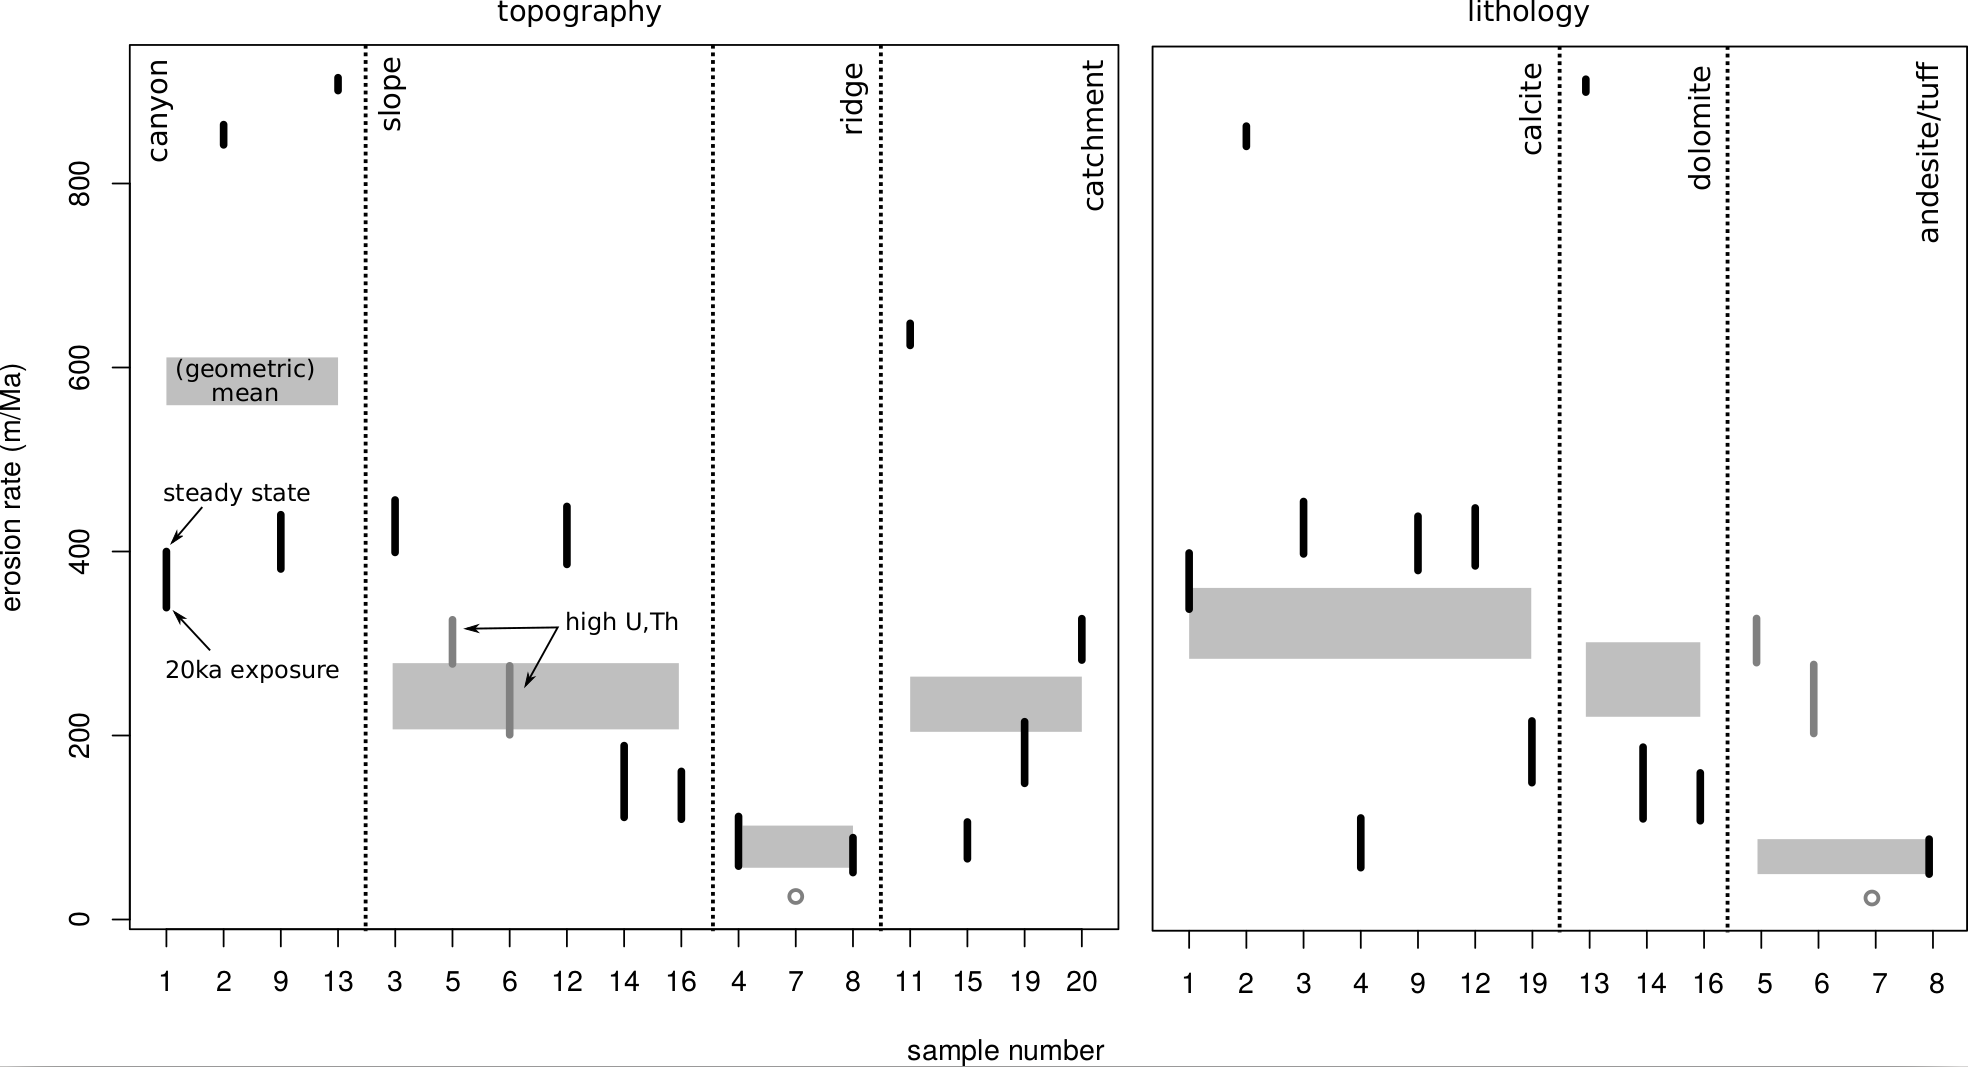
\includegraphics[width=\textwidth]{comparison.png}
  \caption{\textsuperscript{36}Cl-based apparent erosion rates for the
    Allchar area grouped according to topographic location (left) and
    lithology (right). Vertical bars connect the erosion rate
    estimates assuming steady-state (top) and a 20~ka exposure history
    (bottom), respectively. Similarly, the geometric mean erosion
    rates are shown as boxes whose top and bottom margins correspond
    to the steady-state and finite exposure scenarios. Samples~5 and 6
    contain high concentrations of thermal neutron-producing U and Th
    for which an erosion rate can only be calculated under the
    assumption of an unrealistic zero crystallisation age.  Sample~7
    contains too much \textsuperscript{36}Cl to be compatible with the
    20~ka exposure scenario.}
  \label{fig:comparison}
\end{figure}


As expected from the sampling strategy outlined in
Section~\ref{sec:methods}, samples collected from ridges exhibit the
lowest erosion rates, with values ranging from 25 to 112~m/Ma and
geometric\footnote{The geometric mean is used because it is the
  natural average for strictly positive values and is less sensitive
  to outliers than the arithmetic mean.}  mean values of 54 and
100~m/Ma for the 20~ka exposure and steady-state erosion histories,
respectively. In contrast, the bottom of small canyons hosting minor
tributaries of the Majdan River exhibit the highest erosion rates
(range: 339-915~m/Ma, means: 559-611~m/Ma).\\

Samples collected from the slopes between the ridges and the canyon
bottoms are characterised by intermediate erosion rates (range:
109-456~m/Ma, means: 208-281~m/Ma).  Similarly, catchment-wide erosion
rates based on \textsuperscript{36}Cl in the coarse fraction of modern
sediment samples~11, 15 and 20, as well as bedrock sample~19 collected
at the bottom of the main river channel also yield intermediate
erosion rate estimates (range: 66-648~m/Ma, means: 204-264~m/Ma).\\

Grouping the bedrock samples according to lithology shows that by far
the lowest \textsuperscript{36}Cl-based erosion rate estimates are
observed in the hard andesites of samples~7 and 8 (25-89~m/Ma). At
this point it is useful to recall the observation that the calcite
marble contains an order of magnitude less natural Cl than the
dolomite. This suggests that Cl is lost from dolomite during contact
metamorphism. The low \textsuperscript{35}Cl concentration of the
calcite reduces the importance of the thermal neutron production
pathway of \textsuperscript{36}Cl. We would therefore expect the
dolomite to contain more cosmogenic \textsuperscript{36}Cl per gramme
of Ca (spallation + thermal neutron absorption) than the calcite
(spallation only).  This is indeed what is observed, with geometric
mean erosion rates of 282-358~m/Ma for the marble and 222-303~m/Ma for
the dolomite.\\

The dispersion of the individual estimate around these mean values
(84-864~m/Ma and 109-915~m/Ma, respectively) is admittedly too high to
draw any firm conclusions.  But what is clear is that the effect of
thermal neutrons on the erosion rate estimates is at modest at best,
because the difference between the dolomite and the calcite would be
much greater if it were not.\\

As expected, catchment-wide erosion rates based on
\textsuperscript{10}Be-in-quartz are consistently lower than the
\textsuperscript{36}Cl-based estimates (in either bedrock or
sediment). This indicates that silicate lithologies erode more slowly
than carbonates, a result that is entirely consistent with the
\textsuperscript{36}Cl concentrations in andesite discussed
above. Additionally, it is also useful to contemplate the fact that
half life of \textsuperscript{10}Be is more than four times longer
than that of \textsuperscript{36}Cl. This means that
\textsuperscript{10}Be averages erosion rates over longer time scales
than \textsuperscript{36}Cl.\\

The lower \textsuperscript{10}Be-based erosion rates could also be
taken as evidence for an acceleration of the erosion rates in the
Majdanska River Valley over the past million years. Unfortunately, it
is impossible to assess the likelihood of this interpretation with the
current data.\\

The \textsuperscript{36}Cl concentrations in modern river sediments
range from 69 to 155$\times$10\textsuperscript{3}at/g. This dispersion
should not surprise us given the small size of the area occupied by
carbonate lithologies (13, 11 and 20km\textsuperscript{2} for samples
11, 15 and 20, respectively), which may be insufficient to average the
upstream heterogeneity in erosion rates. This is made worse by the
poor resistence to mechanical abrasion of the carbonate clasts, which
biases the detrital carbonate record to nearby sources.
Contrastingly, the \textsuperscript{10}Be concentrations of the fine
and the coarse fractions of samples 17 and 20 are remarkably
consistent, with four aliquots all containing
67-68$\times$10\textsuperscript{3}at[\textsuperscript{10}Be]/g[SiO\textsubscript{2}].\\

Samples~11 and 15 contain much more \textsuperscript{10}Be. There is
no satisfactory explanation for these values, although two separate
observations cast some doubt on their validity. First, the fact that
only one size fraction was analysed for these samples reflects the
difficulty in finding sufficient high quality quartz for cosmogenic
nuclide analysis in this particular sample. Second, one cannot help
but notice that that samples~11 and 15 were collected immediately
below the lorandite mining area (Figure~\ref{fig:catchments}), which
has seen the greatest anthropogenic disturbance.  In any case, the
striking consistency of the remaining four \textsuperscript{10}Be
erosion rate estimates has led us to accept them as the most
representative values for the long-term erosion rate of the Allchar
area.

\begin{figure}[!ht]
  \centering
  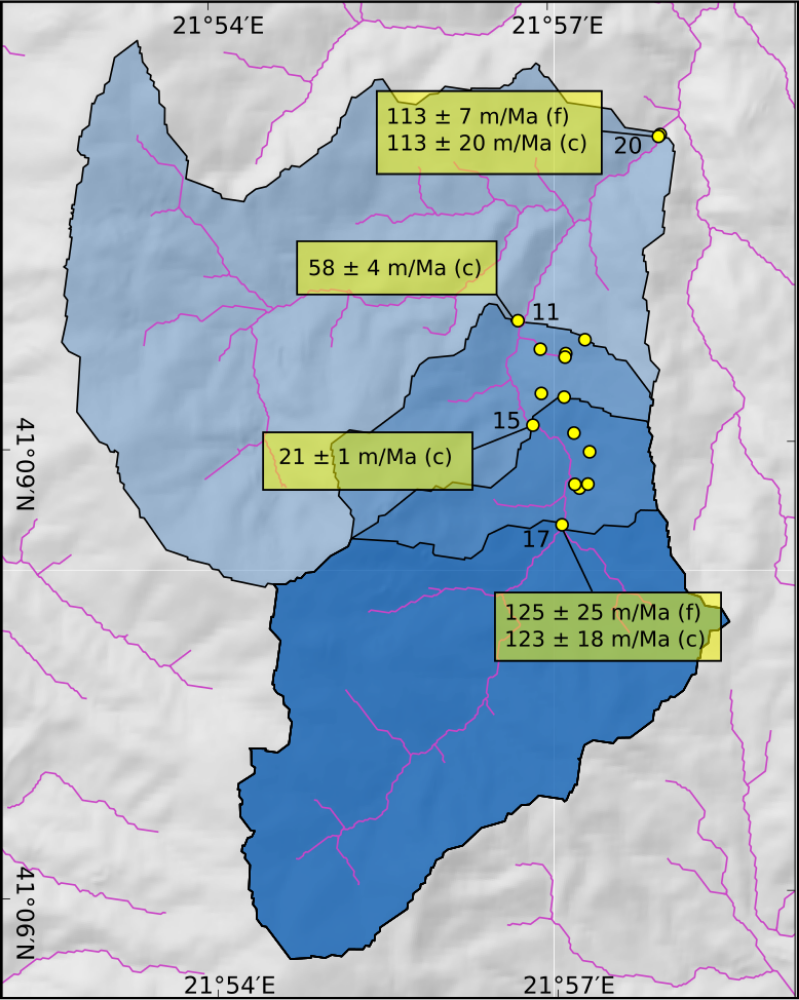
\includegraphics[width=.4\textwidth]{catchments.pdf}
  \caption{Catchment area of the Majdan River and its tributaries
    upstream of the four modern sediment samples, with indication of
    the \textsuperscript{10}Be-based catchment-wide erosion rate
    estimates. (c) refers to the coarse and (f) to the fine fraction.}
  \label{fig:catchments}
\end{figure}

\section{Conclusions}
\label{sec:conclusion}

This study has re-evaluated the erosion rate of the Majdanska River
Valley in southern Macedonia using cosmogenic \textsuperscript{36}Cl
in carbonates from bedrock and modern river sediment, and
\textsuperscript{10}Be in fluvial quartz.  Bedrock samples exhibit the
greatest range of erosion rate estimates, from 51 to 915~m/Ma,
reflecting the small scale variability of erosion rates in both time
and space.\\

The order of magnitude range in erosion rates obtained from our study
is not surprising. It is a result of our sampling strategy, which
specifically targeted the fastest (canyons) and slowest (ridges)
landforms. This is a very different situation from the study of
\citet{pavicevic2016}. Their results exhibit a similar degree of
dispersion to ours, but for unclear reasons.\\

In the presence of the observed levels of dispersion, it would be
unwise to rely on a single sample of bedrock to determine the erosion
rate for the entire Allchar area, as was done by \citet{dockhorn1991}.
Samples collected on ridges, in canyons, and in the anthropogenically
disturbed Crven Dol and Centralni Deo mining areas are unlikely to
yield reliable erosion rates. Carbonate samples collected on slopes
and in the Majdan River yield mutually consistent steady-state erosion
values of 260-280~m/Ma.\\

\textsuperscript{10}Be-derived catchment-wide erosion rate estimates
for samples~17 and 20 are similarly consistent but significantly lower
at 113-125 ~m/Ma, again assuming an erosional steady-state.  These
samples were collected upstream and downstream of the lorandite mining
area, respectively, and constrain the erosion rate of the
quartz-bearing lithologies in the Majdanska River Valley, which occupy
roughly twice as much of the draining area as the carbonate
lithologies.\\

The factor of two difference between the carbonate and silicate
erosion rates is entirely consistent with the local geology and
geomorphology.  Closer inspection of the topographic and geologic maps
(Figure~\ref{fig:maps}) reveals that the quartz-bearing lithologies
(sandstone, gneiss and rhyolite) occupy the higher elevations, whereas
the limestones are found in the valleys.\\

The Pliocene volcanics are currently found on either side of the
Majdanska River Valley, at altitudes of more than 850m, where they
form a hard protective cap on top of the much softer Triassic
carbonates. It is likely that these Pliocene deposits once filled the
valley itself, until they were removed by fluvial or fluvioglacial
erosion. Once the Majdanska River cut through this hard layer and
reached the comparably soft carbonates, erosion would have accelerated
to produce the deep valley that is currently observed.  Under this
scenario, the \textsuperscript{10}Be-based erosion rates represent the
pre-incision values, whereas the \textsuperscript{36}Cl-based erosion
rates represent the current erosion rates of the carbonate areas.\\

Conservatively extrapolating the \textsuperscript{10}Be-derived values
of 100-120~m/Ma over the 4.3~Ma lifespan of the lorandite deposit at
Allchar would suggest the removal of $>450$~m of overburden.  Adding
this amount of shielding to the present 120~m depth of the lorandite
deposit would reduce the effect of the muogenic $^{205}$Pb
contribution sufficiently to be able to see the neutrinogenic
component.\\

Importantly, a recent acceleration of the erosion rate as implied by
the \textsuperscript{36}Cl measurements would further improve the
prospects for the lorandite neutrino detector.  This is because such
an acceleration would mean that the lorandite spent most of its
existence at greater depths, only to be exhumed to the surface
relatively recently.\\

Jointly considering the entire body of our twenty-five new erosion
rate estimates provides sufficient evidence to discard the single
\textsuperscript{36}Cl measurement of \citet{dockhorn1991}. We would
therefore urge the physics community to re-evaluate the feasibility of
the lorandite project. Much work remains to be done to make Melvin
Freedman's vision a reality \citep{pavicevic2012}.  But given the
unique advantages of the geological neutrino detector, we would argue
that the geological neutrino detector certainly deserves a second
chance.

\section*{Authors' contributions}

PV conceived the study, obtained the funding, carried out the field
work and wrote the paper, MR carried out the fieldwork and the sample
analyses, IS and LB contributed to the sample analyses and the data
interpretation, the ASTER team carried out the AMS measurements.

\section*{Funding}

This research was supported by Leverhulme Grant \#RPG-2014-410.

\section*{Acknowledgments}

PV would like to thank Prof. G\"{u}nther Korschinek and an anonymous
referee for feedback on the submitted manuscript.

%\bibliographystyle{/home/pvermees/Dropbox/abbrvplainnat}
%\bibliography{/home/pvermees/Dropbox/biblio}

\begin{thebibliography}{25}
\providecommand{\natexlab}[1]{#1}
\providecommand{\url}[1]{\texttt{#1}}
\expandafter\ifx\csname urlstyle\endcsname\relax
  \providecommand{\doi}[1]{doi: #1}\else
  \providecommand{\doi}{doi: \begingroup \urlstyle{rm}\Url}\fi

\bibitem[Alfimov and Ivy-Ochs(2009)]{alfimov2009}
Alfimov, V. and Ivy-Ochs, S.
\newblock How well do we understand production of $^{36}${C}l in limestone and
  dolomite?
\newblock \emph{Quaternary Geochronology}, 4\penalty0 (6):\penalty0 462 -- 474,
  2009.
\newblock ISSN 1871-1014.
\newblock \doi{DOI: 10.1016/j.quageo.2009.08.005}.
\newblock Advances in Cosmogenic Isotope Research from CRONUS-EU.

\bibitem[Allen et~al.(2012)Allen, Johnson, Heumann, Gooley, and
  Gallin]{allen2012}
Allen, J.~L., Johnson, C.~L., Heumann, M.~J., Gooley, J., and Gallin, W.
\newblock {New technology and methodology for assessing sandstone composition:
  A preliminary case study using a quantitative electron microscope scanner
  (QEMScan)}.
\newblock \emph{Geological Society of America Special Papers}, 487:\penalty0
  177--194, 2012.

\bibitem[Arnold et~al.(2010)Arnold, Merchel, Bourl{\`e}s, Braucher, Benedetti,
  Finkel, Auma{\^\i}tre, Gottdang, and Klein]{arnold2010}
Arnold, M., Merchel, S., Bourl{\`e}s, D.~L., Braucher, R., Benedetti, L.,
  Finkel, R.~C., Auma{\^\i}tre, G., Gottdang, A., and Klein, M.
\newblock {The French accelerator mass spectrometry facility ASTER: improved
  performance and developments}.
\newblock \emph{Nuclear Instruments and Methods in Physics Research Section B:
  Beam Interactions with Materials and Atoms}, 268\penalty0 (11-12):\penalty0
  1954--1959, 2010.

\bibitem[Arnold et~al.(2013)Arnold, Auma{\^\i}tre, Bourl{\`e}s, Keddadouche,
  Braucher, Finkel, Nottoli, Benedetti, and Merchel]{arnold2013}
Arnold, M., Auma{\^\i}tre, G., Bourl{\`e}s, D.~L., Keddadouche, K., Braucher,
  R., Finkel, R.~C., Nottoli, E., Benedetti, L., and Merchel, S.
\newblock {The French accelerator mass spectrometry facility ASTER after 4
  years: Status and recent developments on $^{36}$Cl and $^{129}$I}.
\newblock \emph{Nuclear Instruments and Methods in Physics Research Section B:
  Beam Interactions with Materials and Atoms}, 294:\penalty0 24--28, 2013.

\bibitem[{Bahcall} et~al.(1996){Bahcall}, {Calaprice}, {McDonald}, and
  {Totsuka}]{bahcall1996}
{Bahcall}, J.~N., {Calaprice}, F., {McDonald}, A.~B., and {Totsuka}, Y.
\newblock {Solar neutrino experiments: The next generation}.
\newblock \emph{Physics Today}, 49:\penalty0 30--38, 1996.
\newblock \doi{10.1063/1.881501}.

\bibitem[Bierman et~al.(1995)Bierman, Gillespie, Caffee, and
  Elmore]{bierman1995}
Bierman, P., Gillespie, A., Caffee, M., and Elmore, D.
\newblock {Estimating erosion rates and exposure ages with $^{36}$Cl produced
  by neutron activation}.
\newblock \emph{Geochimica et Cosmochimica Acta}, 59\penalty0 (18):\penalty0
  3779--3798, 1995.

\bibitem[{Dockhorn} et~al.(1991){Dockhorn}, {Neumaier}, {Hartmann},
  {Petitjean}, {Faestermann}, {Korschinek}, {Morinaga}, and
  {Nolte}]{dockhorn1991}
{Dockhorn}, B., {Neumaier}, S., {Hartmann}, F.~J., {Petitjean}, C.,
  {Faestermann}, H., {Korschinek}, G., {Morinaga}, H., and {Nolte}, E.
\newblock {Determination of erosion rates with cosmic ray produced $^{36}$Cl}.
\newblock \emph{Zeitschrift fur Physik A Hadrons and Nuclei}, 341:\penalty0
  117--119, 1991.
\newblock \doi{10.1007/BF01281283}.

\bibitem[Fink et~al.(2000)Fink, Vogt, and Hotchkis]{fink2000}
Fink, D., Vogt, S., and Hotchkis, M.
\newblock {Cross-sections for $^{36}$Cl from Ti at E$_p$= 35--150 MeV:
  applications to in-situ exposure dating}.
\newblock \emph{Nuclear Instruments and Methods in Physics Research Section B:
  Beam Interactions with Materials and Atoms}, 172\penalty0 (1):\penalty0
  861--866, 2000.

\bibitem[{Freedman} et~al.(1976){Freedman}, {Stevens}, {Horwitz}, {Fuchs},
  {Lerner}, {Goodman}, {Childs}, and {Hessler}]{freedman1976}
{Freedman}, M.~S., {Stevens}, C.~M., {Horwitz}, E.~P., {Fuchs}, L.~H.,
  {Lerner}, J.~L., {Goodman}, L.~S., {Childs}, W.~J., and {Hessler}, J.
\newblock {Solar neutrinos - Proposal for a new test}.
\newblock \emph{Science}, 193:\penalty0 1117--1119, 1976.
\newblock \doi{10.1126/science.193.4258.1117}.

\bibitem[Jarvis et~al.(2008)Jarvis, Reuter, Nelson, Guevara,
  et~al.]{jarvis2008}
Jarvis, A., Reuter, H.~I., Nelson, A., Guevara, E., et~al.
\newblock {Hole-filled SRTM for the globe Version 4}.
\newblock \emph{available from the CGIAR-CSI SRTM 90m Database (http://srtm.
  csi. cgiar. org)}, 15, 2008.

\bibitem[Menkovic et~al.(2004)Menkovic, Markovic, Cupkovic, Pavlovic, Trivic,
  and Banjac]{menkovic2004}
Menkovic, L., Markovic, M., Cupkovic, T., Pavlovic, R., Trivic, B., and Banjac,
  N.
\newblock {Glacial morphology of Serbia, with comments on the Pleistocene
  Glaciation of Monte Negro, Macedonia and Albania}.
\newblock \emph{Developments in Quaternary Sciences}, 2:\penalty0 379--384,
  2004.

\bibitem[Merchel et~al.(2008)Merchel, Arnold, Auma{\^\i}tre, Benedetti,
  Bourl{\`e}s, Braucher, Alfimov, Freeman, Steier, and Wallner]{merchel2008}
Merchel, S., Arnold, M., Auma{\^\i}tre, G., Benedetti, L., Bourl{\`e}s, D.,
  Braucher, R., Alfimov, V., Freeman, S., Steier, P., and Wallner, A.
\newblock Towards more precise $^{10}${B}e and $^{36}${C}l data from
  measurements at the 10$^{-14}$ level: Influence of sample preparation.
\newblock \emph{Nuclear Instruments and Methods in Physics Research Section B:
  Beam Interactions with Materials and Atoms}, 266\penalty0 (22):\penalty0
  4921--4926, 2008.

\bibitem[{Neubauer} et~al.(2009){Neubauer}, {Pavi{\'c}evi{\'c}}, {Genser},
  {Jelenkovi{\'c}}, {Boev}, and {Amthauer}]{neubauer2009}
{Neubauer}, F., {Pavi{\'c}evi{\'c}}, M.~K., {Genser}, J., {Jelenkovi{\'c}}, R.,
  {Boev}, B., and {Amthauer}, G.
\newblock {$^{40}$Ar/$^{39}$Ar dating of geological events of the Allchar
  deposit and its host rocks}.
\newblock \emph{Geochimica et Cosmochimica Acta Supplement}, 73:\penalty0 938,
  2009.

\bibitem[{Neumaier} et~al.(1991){Neumaier}, {Nolte}, and
  {Morinaga}]{neumaier1991}
{Neumaier}, S., {Nolte}, E., and {Morinaga}, H.
\newblock {Feasibility studies of the geochemical solar neutrino experiment
  $^{205}$Tl($\nu$,$e^{‑}$)$^{205}$Pb$^*$}.
\newblock \emph{Zeitschrift fur Physik A Hadrons and Nuclei}, 340:\penalty0
  415--418, 1991.
\newblock \doi{10.1007/BF01290330}.

\bibitem[{Pavi{\'c}evi{\'c}}(1988)]{pavicevic1988}
{Pavi{\'c}evi{\'c}}, M.~K.
\newblock {Lorandite from Allchar - A low energy solar neutrino dosimeter}.
\newblock \emph{Nuclear Instruments and Methods in Physics Research A},
  271:\penalty0 287--296, 1988.
\newblock \doi{10.1016/0168-9002(88)90171-4}.

\bibitem[Pavi{\'c}evi{\'c} et~al.(2012)Pavi{\'c}evi{\'c}, Bosch, Amthauer,
  Ani{\v{c}}in, Boev, Br{\"u}chle, Cvetkovi{\'c}, Djur{\v{c}}i{\'c}, Henning,
  Jelenkovi{\'c}, et~al.]{pavicevic2012}
Pavi{\'c}evi{\'c}, M., Bosch, F., Amthauer, G., Ani{\v{c}}in, I., Boev, B.,
  Br{\"u}chle, W., Cvetkovi{\'c}, V., Djur{\v{c}}i{\'c}, Z., Henning, W.,
  Jelenkovi{\'c}, R., et~al.
\newblock {Status and New Data of the Geochemical Determination of the
  pp-Neutrino Flux by LOREX}.
\newblock \emph{Advances in High Energy Physics}, 2012, 2012.

\bibitem[Pavi{\'c}evi{\'c} et~al.(2016)Pavi{\'c}evi{\'c}, Cvetkovi{\'c},
  Niedermann, Pejovi{\'c}, Amthauer, Boev, Bosch, Ani{\v{c}}in, and
  Henning]{pavicevic2016}
Pavi{\'c}evi{\'c}, M., Cvetkovi{\'c}, V., Niedermann, S., Pejovi{\'c}, V.,
  Amthauer, G., Boev, B., Bosch, F., Ani{\v{c}}in, I., and Henning, W.
\newblock {Erosion rate study at the Allchar deposit (Macedonia) based on
  radioactive and stable cosmogenic nuclides ($^{26}$Al, $^{36}$Cl, $^{3}$He,
  and $^{21}$Ne)}.
\newblock \emph{Geochemistry, Geophysics, Geosystems}, 2016.

\bibitem[Schimmelpfennig et~al.(2009)Schimmelpfennig, Benedetti, Finkel, Pik,
  Blard, Bourl{\`e}s, Burnard, and Williams]{schimmelpfennig2009}
Schimmelpfennig, I., Benedetti, L., Finkel, R., Pik, R., Blard, P.-H.,
  Bourl{\`e}s, D., Burnard, P., and Williams, A.
\newblock Sources of in-situ $^{36}${C}l in basaltic rocks. implications for
  calibration of production rates.
\newblock \emph{Quaternary Geochronology}, 4\penalty0 (6):\penalty0 441--461,
  2009.

\bibitem[Schimmelpfennig et~al.(2011)Schimmelpfennig, Benedetti, Garreta, Pik,
  Blard, Burnard, Bourles, Finkel, Ammon, and Dunai]{schimmelpfennig2011}
Schimmelpfennig, I., Benedetti, L., Garreta, V., Pik, R., Blard, P.-H.,
  Burnard, P., Bourles, D., Finkel, R., Ammon, K., and Dunai, T.
\newblock {Calibration of cosmogenic $^{36}$Cl production rates from Ca and K
  spallation in lava flows from Mt. Etna (38$^\circ$N, Italy) and Payun Matru
  (36$^\circ$S, Argentina)}.
\newblock \emph{Geochimica et Cosmochimica Acta}, 75\penalty0 (10):\penalty0
  2611--2632, 2011.

\bibitem[Schimmelpfennig et~al.(2014)Schimmelpfennig, Schaefer, Putnam,
  Koffman, Benedetti, IVY-OCHS, Team, and Schl{\"u}chter]{schimmelpfennig2014}
Schimmelpfennig, I., Schaefer, J.~M., Putnam, A.~E., Koffman, T., Benedetti,
  L., IVY-OCHS, S., Team, A., and Schl{\"u}chter, C.
\newblock {36Cl production rate from K-spallation in the European Alps
  (Chironico landslide, Switzerland)}.
\newblock \emph{Journal of Quaternary Science}, 29\penalty0 (5):\penalty0
  407--413, 2014.

\bibitem[Stone(2000)]{stone2000}
Stone, J.~O.
\newblock Air pressure and cosmogenic isotope production.
\newblock \emph{Journal of Geophysical Research}, 105:\penalty0 23,753--23,759,
  2000.

\bibitem[Stone et~al.(1998)Stone, Evans, Fifield, Allan, and
  Cresswell]{stone1998}
Stone, J., Evans, J., Fifield, L., Allan, G., and Cresswell, R.
\newblock Cosmogenic chlorine-36 production in calcite by muons.
\newblock \emph{Geochimica et Cosmochimica Acta}, 62\penalty0 (3):\penalty0
  433--454, 1998.

\bibitem[Stone et~al.(2005)Stone, Fifield, and Vasconcelos]{stone2005}
Stone, J.~O., Fifield, K., and Vasconcelos, P.
\newblock {Terrestrial Chlorine-36 production from spallation of iron}.
\newblock In \emph{Abstract of 10th International Conference on Accelerator
  Mass Spectrometry}. Berkeley California, 2005.

\bibitem[{Vermeesch}(2007)]{vermeesch2007c}
{Vermeesch}, P.
\newblock {CosmoCalc: An Excel add-in for cosmogenic nuclide calculations}.
\newblock \emph{Geochemistry, Geophysics, Geosystems}, 8:\penalty0 8003, 2007.
\newblock \doi{10.1029/2006GC001530}.

\bibitem[{von Blanckenburg}(2005)]{vonblanckenburg2005}
{von Blanckenburg}, F.
\newblock {The control mechanisms of erosion and weathering at basin scale from
  cosmogenic nuclides in river sediment}.
\newblock \emph{Earth and Planetary Science Letters}, 237:\penalty0 462--479,
  2005.
\newblock \doi{10.1016/j.epsl.2005.06.030}.

\end{thebibliography}

\end{document}
